\definecolor{tiffanyblue}{RGB}{129,216,208}
\definecolor{bangdiblue}{RGB}{0,149,182}
\definecolor{kleinblue}{RGB}{0,47,167}
\definecolor{kabuliblue}{RGB}{26,85,153}
\definecolor{purple}{RGB}{138,43,226}

\begin{figure}[t!]
  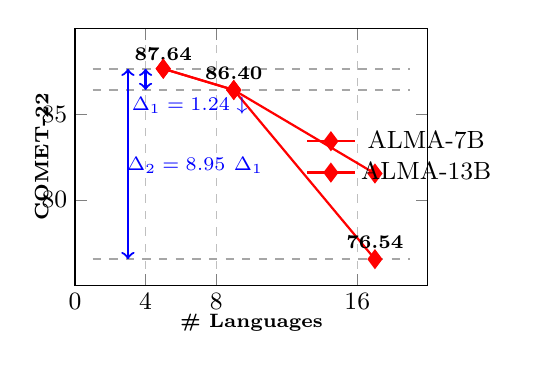
\begin{tikzpicture}
  \pgfplotsset{set layers}
    \scriptsize{
    \begin{axis}[
      align=center,
      %ymajorgrids,
      xmajorgrids,
      %axis lines=left,
      grid style={dashed, gray!50},
      width=0.5\textwidth,
      height=.4\textwidth,
      xlabel={\# Languages},
      ylabel={COMET-22},
      xlabel style={font=\bfseries, yshift=0.5em},
      ylabel style={font=\bfseries, yshift=-1.0em},
      yticklabel style={font=\small},
      xticklabel style={font=\small},
      ymin=75, ymax=90, 
      ytick={80, 85},
      xmin=0, xmax=20, 
      xtick={0, 4, 8, 16},
      legend style={
        at={(0.63,0.5)}, anchor=west,
        draw=none, fill=none, font=\small
      },
      % legend cell align={left}
    ]

    % Main data
    \addplot[red, mark=diamond*, mark size=3.0pt, thick, mark options={solid, fill=red}] 
      coordinates {(5, 87.64) (9, 86.40) (17, 76.54)};
    \addlegendentry{ALMA-7B}

    \addplot[red, mark=diamond*, mark size=3.0pt, thick, mark options={solid, fill=red}] 
      coordinates {(5, 87.64) (9, 86.40) (17, 81.53)};
    \addlegendentry{ALMA-13B}

    % Upper reference line
    \addplot[thick, dashed, gray!70] 
      coordinates {(1, 87.64) (19, 87.64)};
    % \addlegendentry{Upper Bound}

    % Lower reference line
    \addplot[thick, dashed, gray!70] 
      coordinates {(1, 76.54) (19, 76.54)};
    % \addlegendentry{Lower Bound}

% Middle reference line
    \addplot[thick, dashed, gray!70] 
      coordinates {(1, 86.40) (19, 86.40)};
    % \addlegendentry{Lower Bound}


    % Add vertical arrow to show difference
    \draw[<->, thick, blue] 
      (axis cs:3, 87.64) -- (axis cs:3, 76.54);


      % Add vertical arrow to show difference
    \draw[<->, thick, blue] 
      (axis cs:4, 87.64) -- (axis cs:4, 86.40);

    % Add difference label
    \node[blue, font=\bfseries] at (axis cs:6.8, 82.0) {$\Delta_2  = 8.95~\Delta_1  $};

    \node[blue, font=\bfseries] at (axis cs:6.5, 85.5) {$\Delta_1 = 1.24 \downarrow$};

    \node[ font=\bfseries] at (axis cs:5, 88.5) {87.64};
    \node[ font=\bfseries] at (axis cs:9, 87.4) {86.40};
    \node[font=\bfseries] at (axis cs:17, 77.54) {76.54};
    
    \end{axis}
    }
  \end{tikzpicture}
\vskip -0.1in
    \caption{The curse of multilinguality. We use high-quality mulit-lingual pararrel data to tune ALMA-7B-Pretrain Model.}
    \label{fig:curse_of_multilinguality}
\end{figure}
